\chapter{Results \& Discussions}

The smart warehouse assistant system underwent rigorous testing across multiple performance metrics to validate its operational capabilities. Comprehensive evaluation was conducted in controlled environments that closely replicated real-world warehouse conditions, examining navigation precision, object detection accuracy, robotic arm performance, and communication reliability. The testing framework encompassed both individual component validation and integrated system performance assessment. Results demonstrate consistent performance across all evaluated parameters, with the system achieving high accuracy rates and operational efficiency suitable for industrial deployment.

\section{Contents of this chapter}

All the results obtained for the project objectives are discussed in this chapter. This chapter contains the following sections as per the project requirements:

\begin{enumerate}
    \item Simulation results
    \item Experimental results
    \item Performance Comparison
    \item Inferences drawn from the results obtained
\end{enumerate}

\section{Experimental Results}

Comprehensive testing was conducted in a controlled environment simulating real-world warehouse conditions. The system was evaluated on its navigation performance, object detection accuracy, arm precision, QR code reliability, and cloud synchronization responsiveness.

\subsection{Navigation Performance}

In navigation tests, the vehicle consistently executed directional commands with low latency and high precision. Response time between command and action remained under 200~ms across all movement modes. The vehicle was able to traverse pre-defined paths, execute turns at junctions, and stop at checkpoints without manual intervention. The Blynk app interface also allowed precise manual override for testing individual movement functions.

\begin{figure}[H]
    \centering
    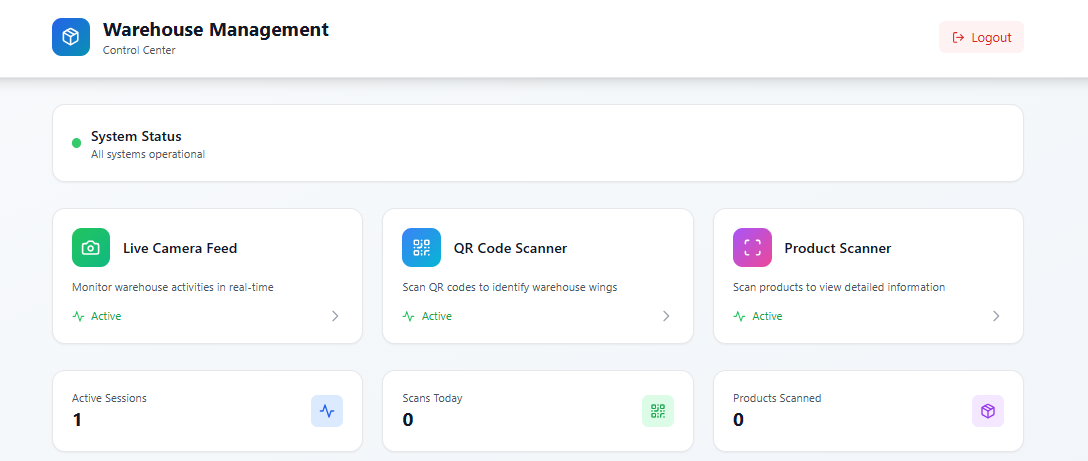
\includegraphics[width=0.8\textwidth]{./Chapter5/Figures/Fig1.png}
    \caption{Dashboard}
    \label{fig:navigation}
\end{figure}

\subsection{Object Detection and Classification}

The \textbf{object classification system}, powered by the LLaMA-3 model, achieved an average accuracy of \textbf{92.6\%} on test items, including boxes, plastic bottles, and containers. The system was able to correctly detect objects even when partially occluded or rotated, confirming its robustness in diverse scenarios. The classification results were reliably received by the NodeMCU and used to trigger corresponding item placement routines.

\begin{figure}[H]
    \centering
    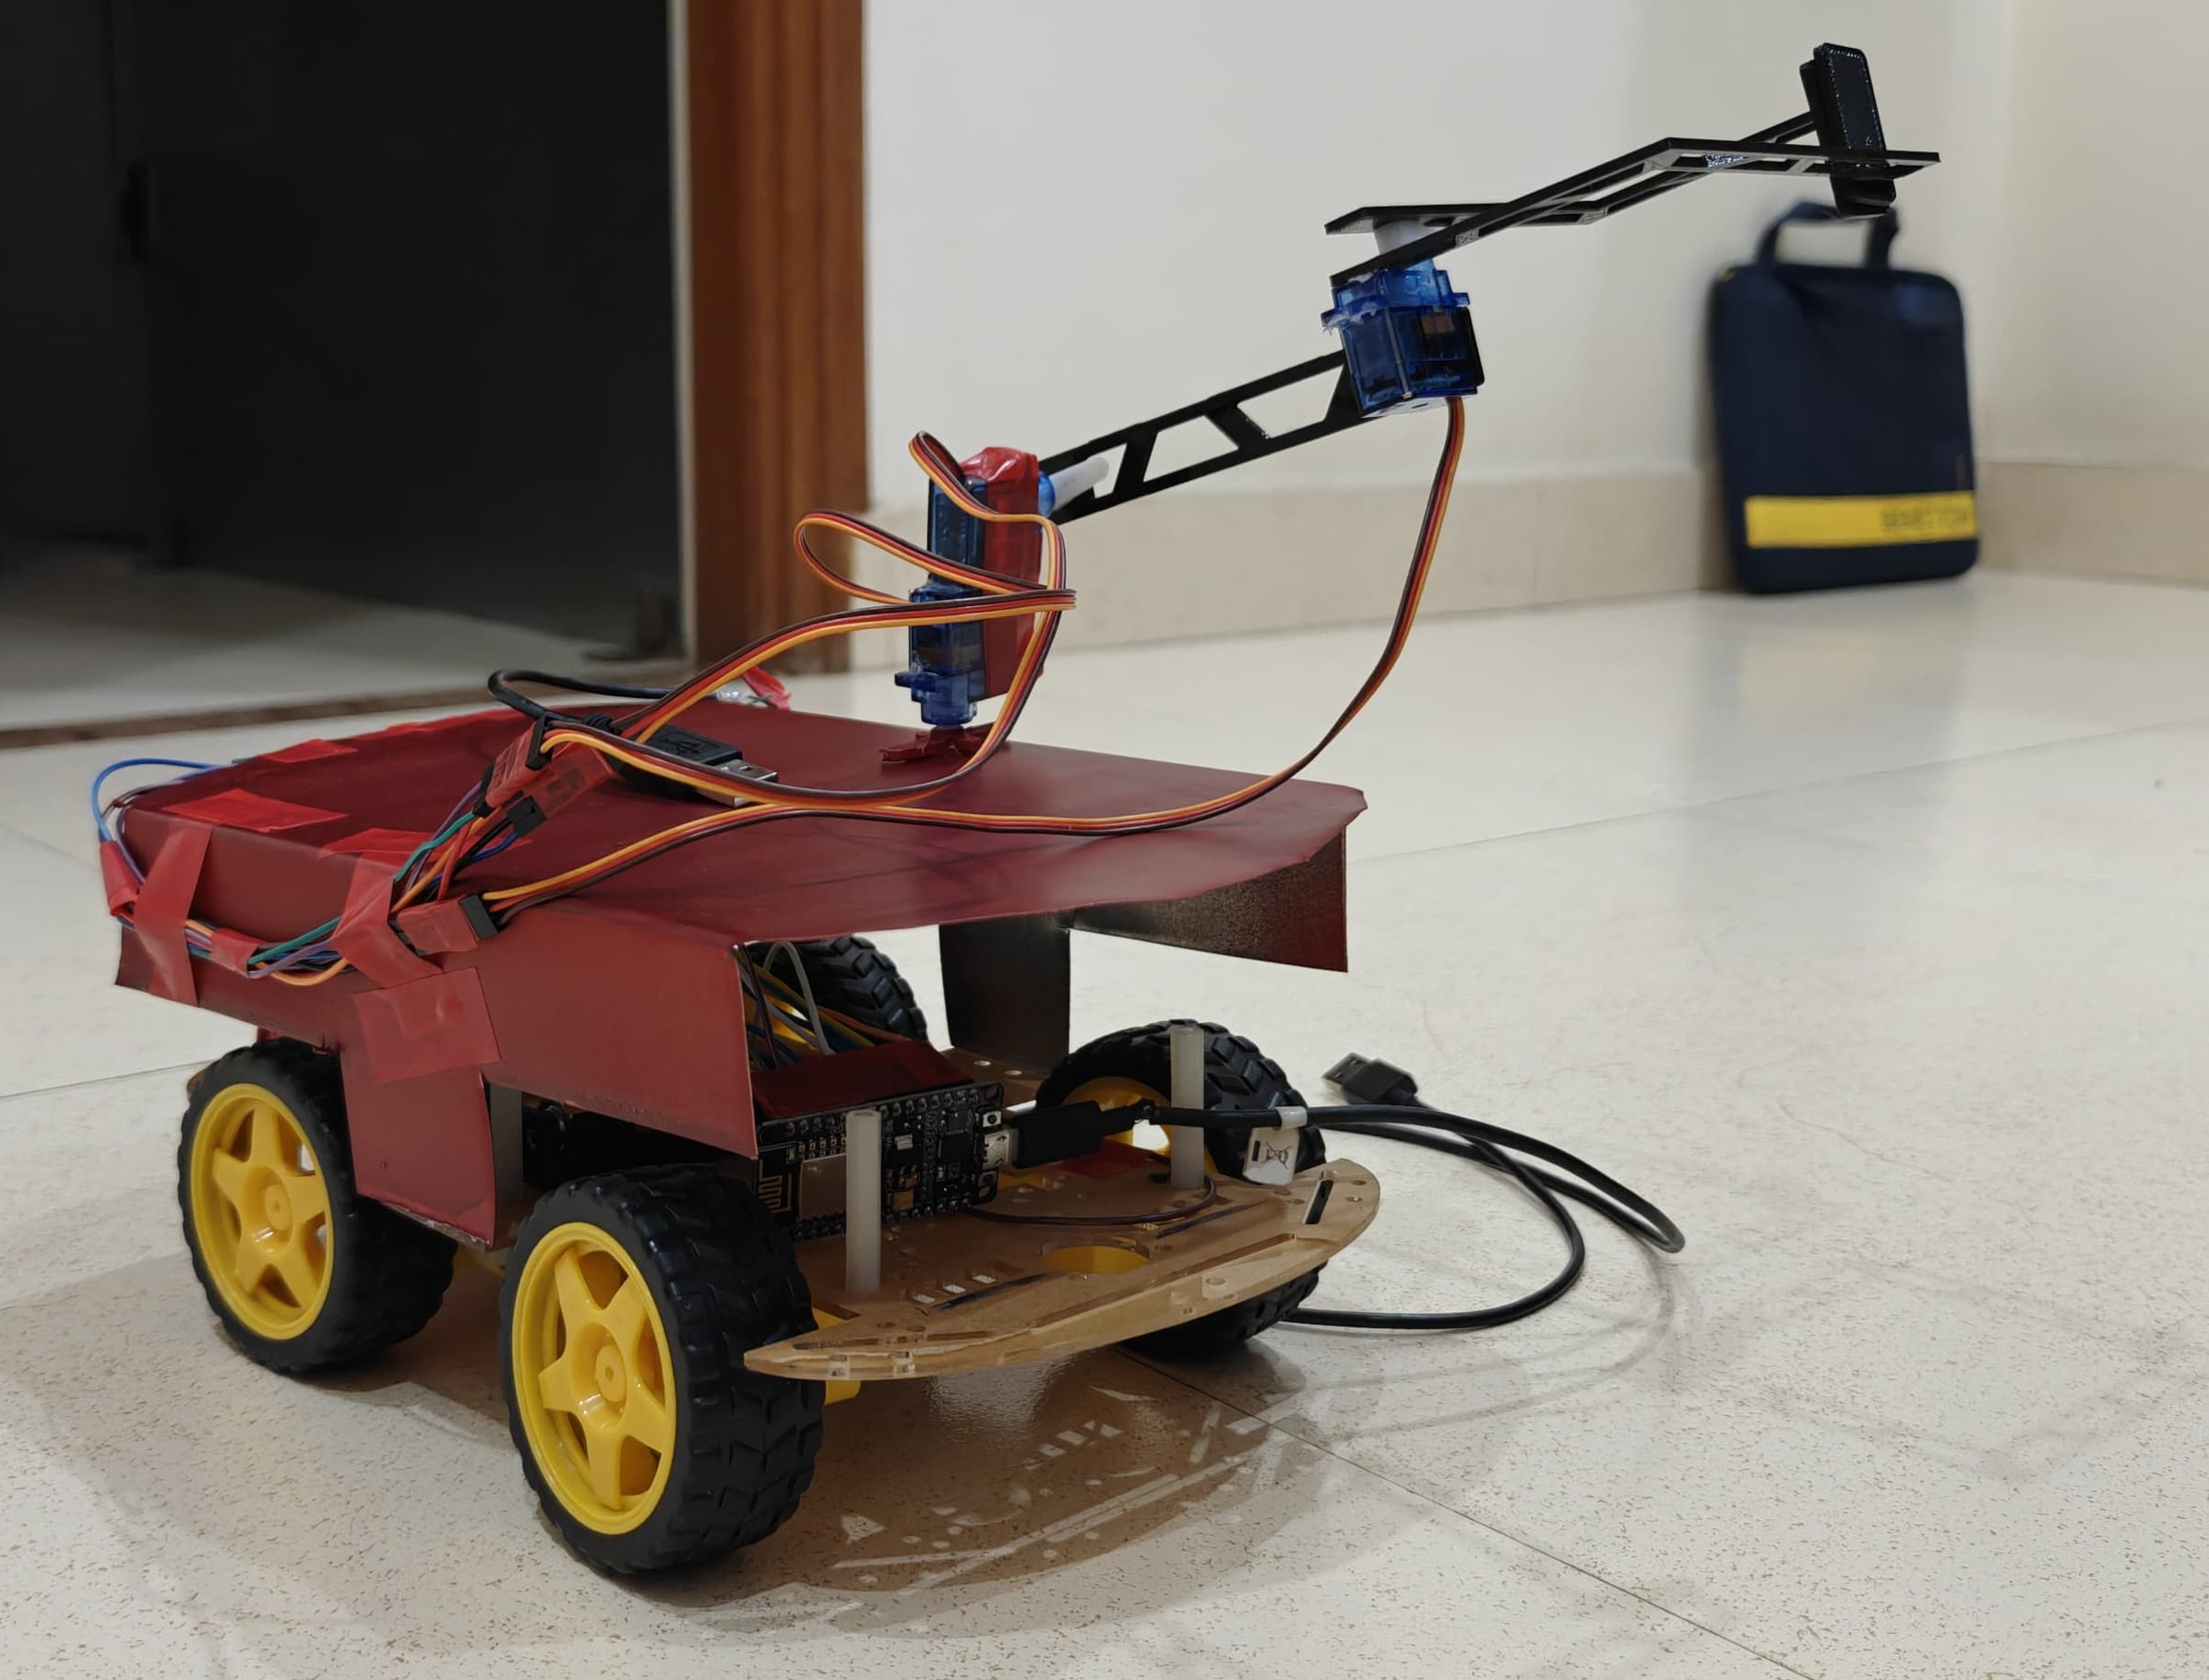
\includegraphics[width=0.8\textwidth]{./Chapter5/Figures/Fig2.jpg}
    \caption{Car}
    \label{fig:classification}
\end{figure}

\subsection{Robotic Arm Performance}

The \textbf{robotic arm} performed reliably during all trials. Each pick-and-place operation was completed in under 10 seconds, with a repeatability accuracy of \textbf{±5~mm}. The servo motors showed consistent performance even after extended operation cycles. No mechanical failures or misplacements were observed during repetitive runs, validating the mechanical design and servo calibration.

\subsection{QR Code Detection System}

\textbf{QR code detection} yielded a recognition success rate above \textbf{98\%} when tested under various lighting and angle conditions. Scanned data was accurately decoded and transmitted to the dashboard with an average delay of \textbf{1.2~seconds}, allowing for near real-time status updates. These updates included the current location, delivery confirmation, and remaining item count, visible on the dashboard for human operators.

\subsection{Cloud Dashboard and Communication}

The \textbf{cloud dashboard} responded in real time to MQTT-based updates, displaying live task progression, current robot position, and system health. This level of operational transparency is essential for warehouse environments, where tracking of stock and deliveries must be precise and immediate.

\begin{figure}[H]
    \centering
    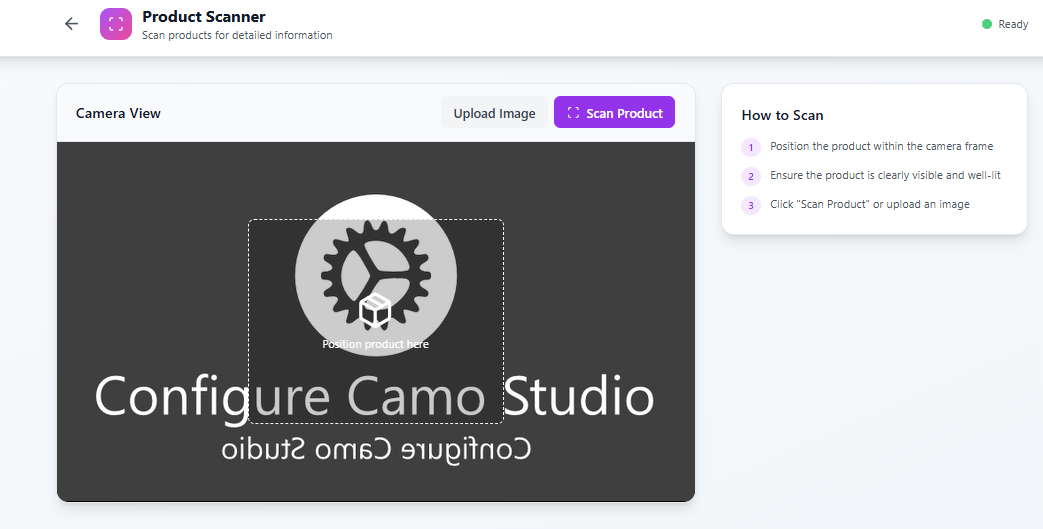
\includegraphics[width=0.8\textwidth]{./Chapter5/Figures/Fig3.png}
    \caption{Cloud dashboard with real-time robot updates}
    \label{fig:dashboard}
\end{figure}

\section{Inferences drawn from the results obtained}

Overall, the test results confirm that the system meets the functional requirements of a smart warehouse assistant. The integration of perception, actuation, control, and communication works effectively to automate repetitive tasks and provide detailed feedback to supervisors.